\chapter{Khảo Sát Và Phân Tích Yêu Cầu}

\section{Khảo sát hiện trạng}
\subsection{Nhu cầu người dùng và Phân tích 5W1H}
Để xác định các tính năng cần có của hệ thống quan trắc chất lượng không khí, nhóm đã tiến hành phân tích nhu cầu của các nhóm đối tượng sử dụng mục tiêu thông qua phương pháp 5W1H. Chi tiết cuộc phân tích được mô tả như sau:
\begin{enumerate}
    \item \textbf{Who (Ai sử dụng?)}: 
    \begin{itemize}
        \item \textit{Người dùng chính}: Học sinh, sinh viên và nhà nghiên cứu trong lĩnh vực kỹ thuật nhúng/IoT cần bộ dữ liệu môi trường thực tế có cấu trúc rõ ràng để thực hành phân tích số liệu, hiệu chỉnh sai số cảm biến hoặc phát triển mô hình dự báo.
        \item \textit{Người dùng phụ nếu như có cơ hội phát triển thành sản phẩm có mục đích thương mại}: Người quản lý phòng học, hộ gia đình hoặc ban quản lý nhà xe cần theo dõi nhanh mức độ ô nhiễm không khí tại vị trí lắp đặt để đưa ra quyết định thông gió hoặc bật quạt hút bảo vệ sức khỏe.
    \end{itemize}
    \item \textbf{What (Hệ thống cung cấp những gì?)}: Một thiết bị phần cứng nhỏ gọn có khả năng hiển thị các chỉ số tại chỗ (OLED), lưu trữ dữ liệu lịch sử trên đám mây, phát tín hiệu cảnh báo tại chỗ (LED/Còi-Buzzer) và đẩy tin nhắn cảnh báo khẩn cấp/báo cáo định kỳ lên điện thoại (Telegram).
    \item \textbf{Where (Hệ thống hoạt động ở đâu?)}: Đặt tại không gian trong nhà (indoor) như phòng học, phòng thí nghiệm, phòng ngủ hoặc khu vực bán lộ thiên như nhà gửi xe (outdoor).
    \item \textbf{When (Khi nào hệ thống hoạt động?)}: Hệ thống đảm bảo có thể hoạt động liên tục 24/7. Cứ mỗi chu kỳ lấy mẫu (mặc định 5 phút), hệ thống sẽ thức dậy, tự động làm nóng cảm biến, đọc giá trị, hiển thị và truyền dữ liệu lên và ghi lại trên cloud.
    \item \textbf{Why (Tại sao cần hệ thống này?)}: Để giúp người dùng nhận biết các thông số xung quanh mình ở thời điểm hiện tại, thay vì theo khu vực khi tra cứu trên internet đồng thời nhận biết được các điều kiện ô nhiễm vô hình một cách trực quan, tránh hít phải khí độc và bụi mịn ở mức nguy hiểm, đồng thời cung cấp chuỗi số liệu thực nghiệm phục vụ học tập, làm project có tính thực tiễn.
    \item \textbf{How (Hệ thống hoạt động như thế nào?)}: ESP32 đọc dữ liệu từ các cảm biến qua giao tiếp Analog/GPIO/I2C, xử lý chống nhiễu lọc trung bình, gửi dữ liệu qua HTTPS POST trực tiếp lên REST API của Supabase và kích hoạt các trigger cảnh báo tự động thông qua webhook.
\end{enumerate}

\subsection{Các nhóm giải pháp hiện có trên thị trường}
Hiện nay, việc theo dõi chất lượng không khí có thể thực hiện qua 3 nhóm giải pháp chính:
\begin{itemize}
    \item \textbf{Trạm quan trắc chuyên dụng chuyên nghiệp (ví dụ: PAMAir, trạm khí tượng của chính phủ)}:
    \begin{figure}[H]
    \centering
    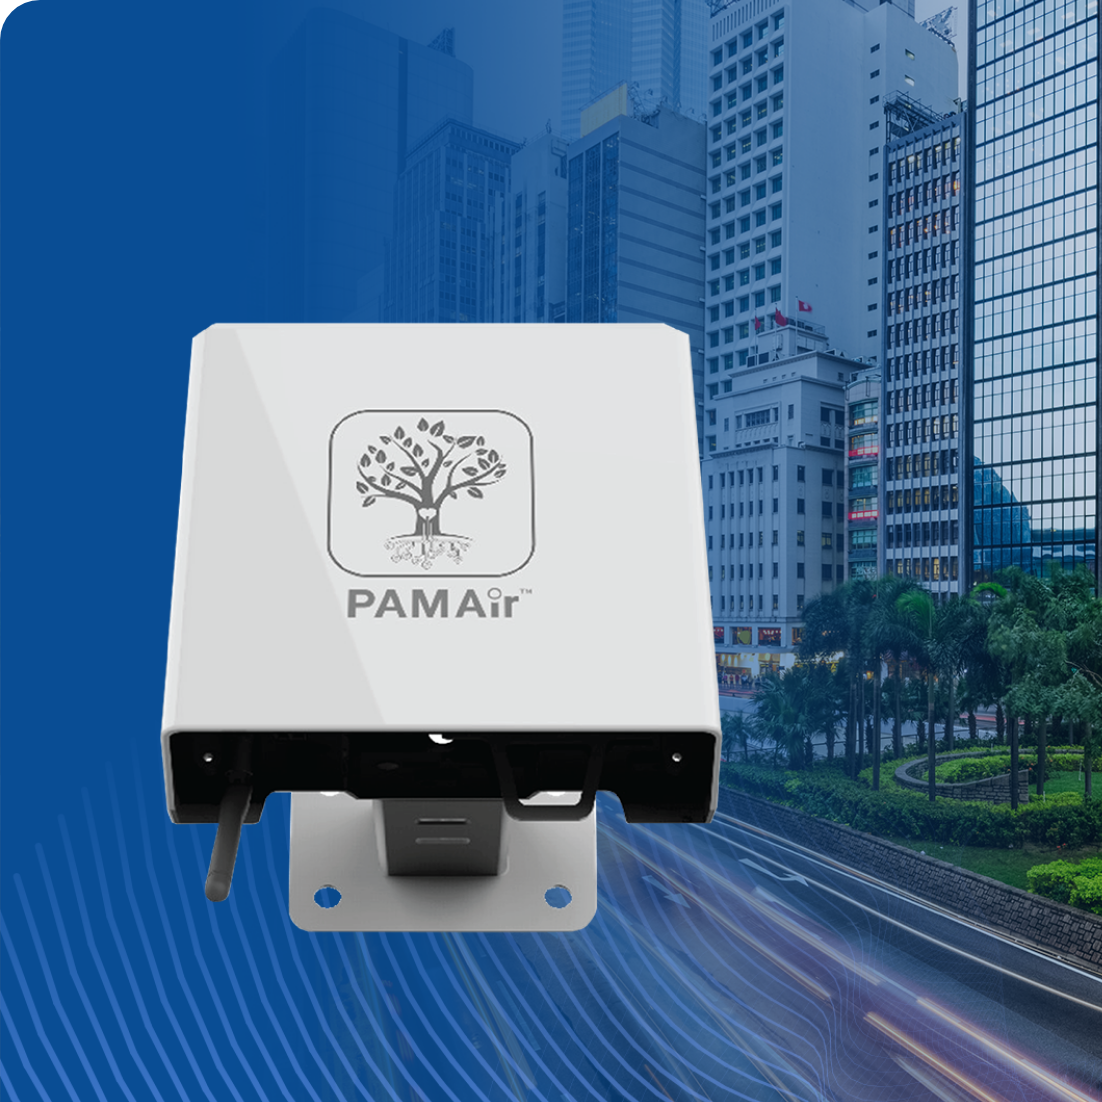
\includegraphics[
        width=0.75\textwidth,
        height=0.28\textheight,
        keepaspectratio
    ]{images/tram_quan_trac_chuyen_dung.png}
    \caption{Ví dụ về trạm quan trắc chất lượng không khí chuyên dụng}
    \label{fig:tramquanthacchuyendung}
\end{figure}
  \begin{itemize}
      \item \textit{Ưu điểm}: Độ chính xác cực kỳ cao, cảm biến đạt chuẩn đo lường quốc gia, hoạt động ổn định trong mọi điều kiện thời tiết khắc nghiệt.
      \item \textit{Hạn chế}: Chi phí đầu tư rất lớn (vài chục đến hàng trăm triệu đồng), thiết kế hệ thống đóng kín, sinh viên không thể can thiệp sâu vào phần cứng hay cấu trúc firmware.
    \end{itemize}
\item \textbf{Thiết bị đo thương mại di động (ví dụ: IQAir AirVisual Pro)}:

\begin{figure}[H]
    \centering
    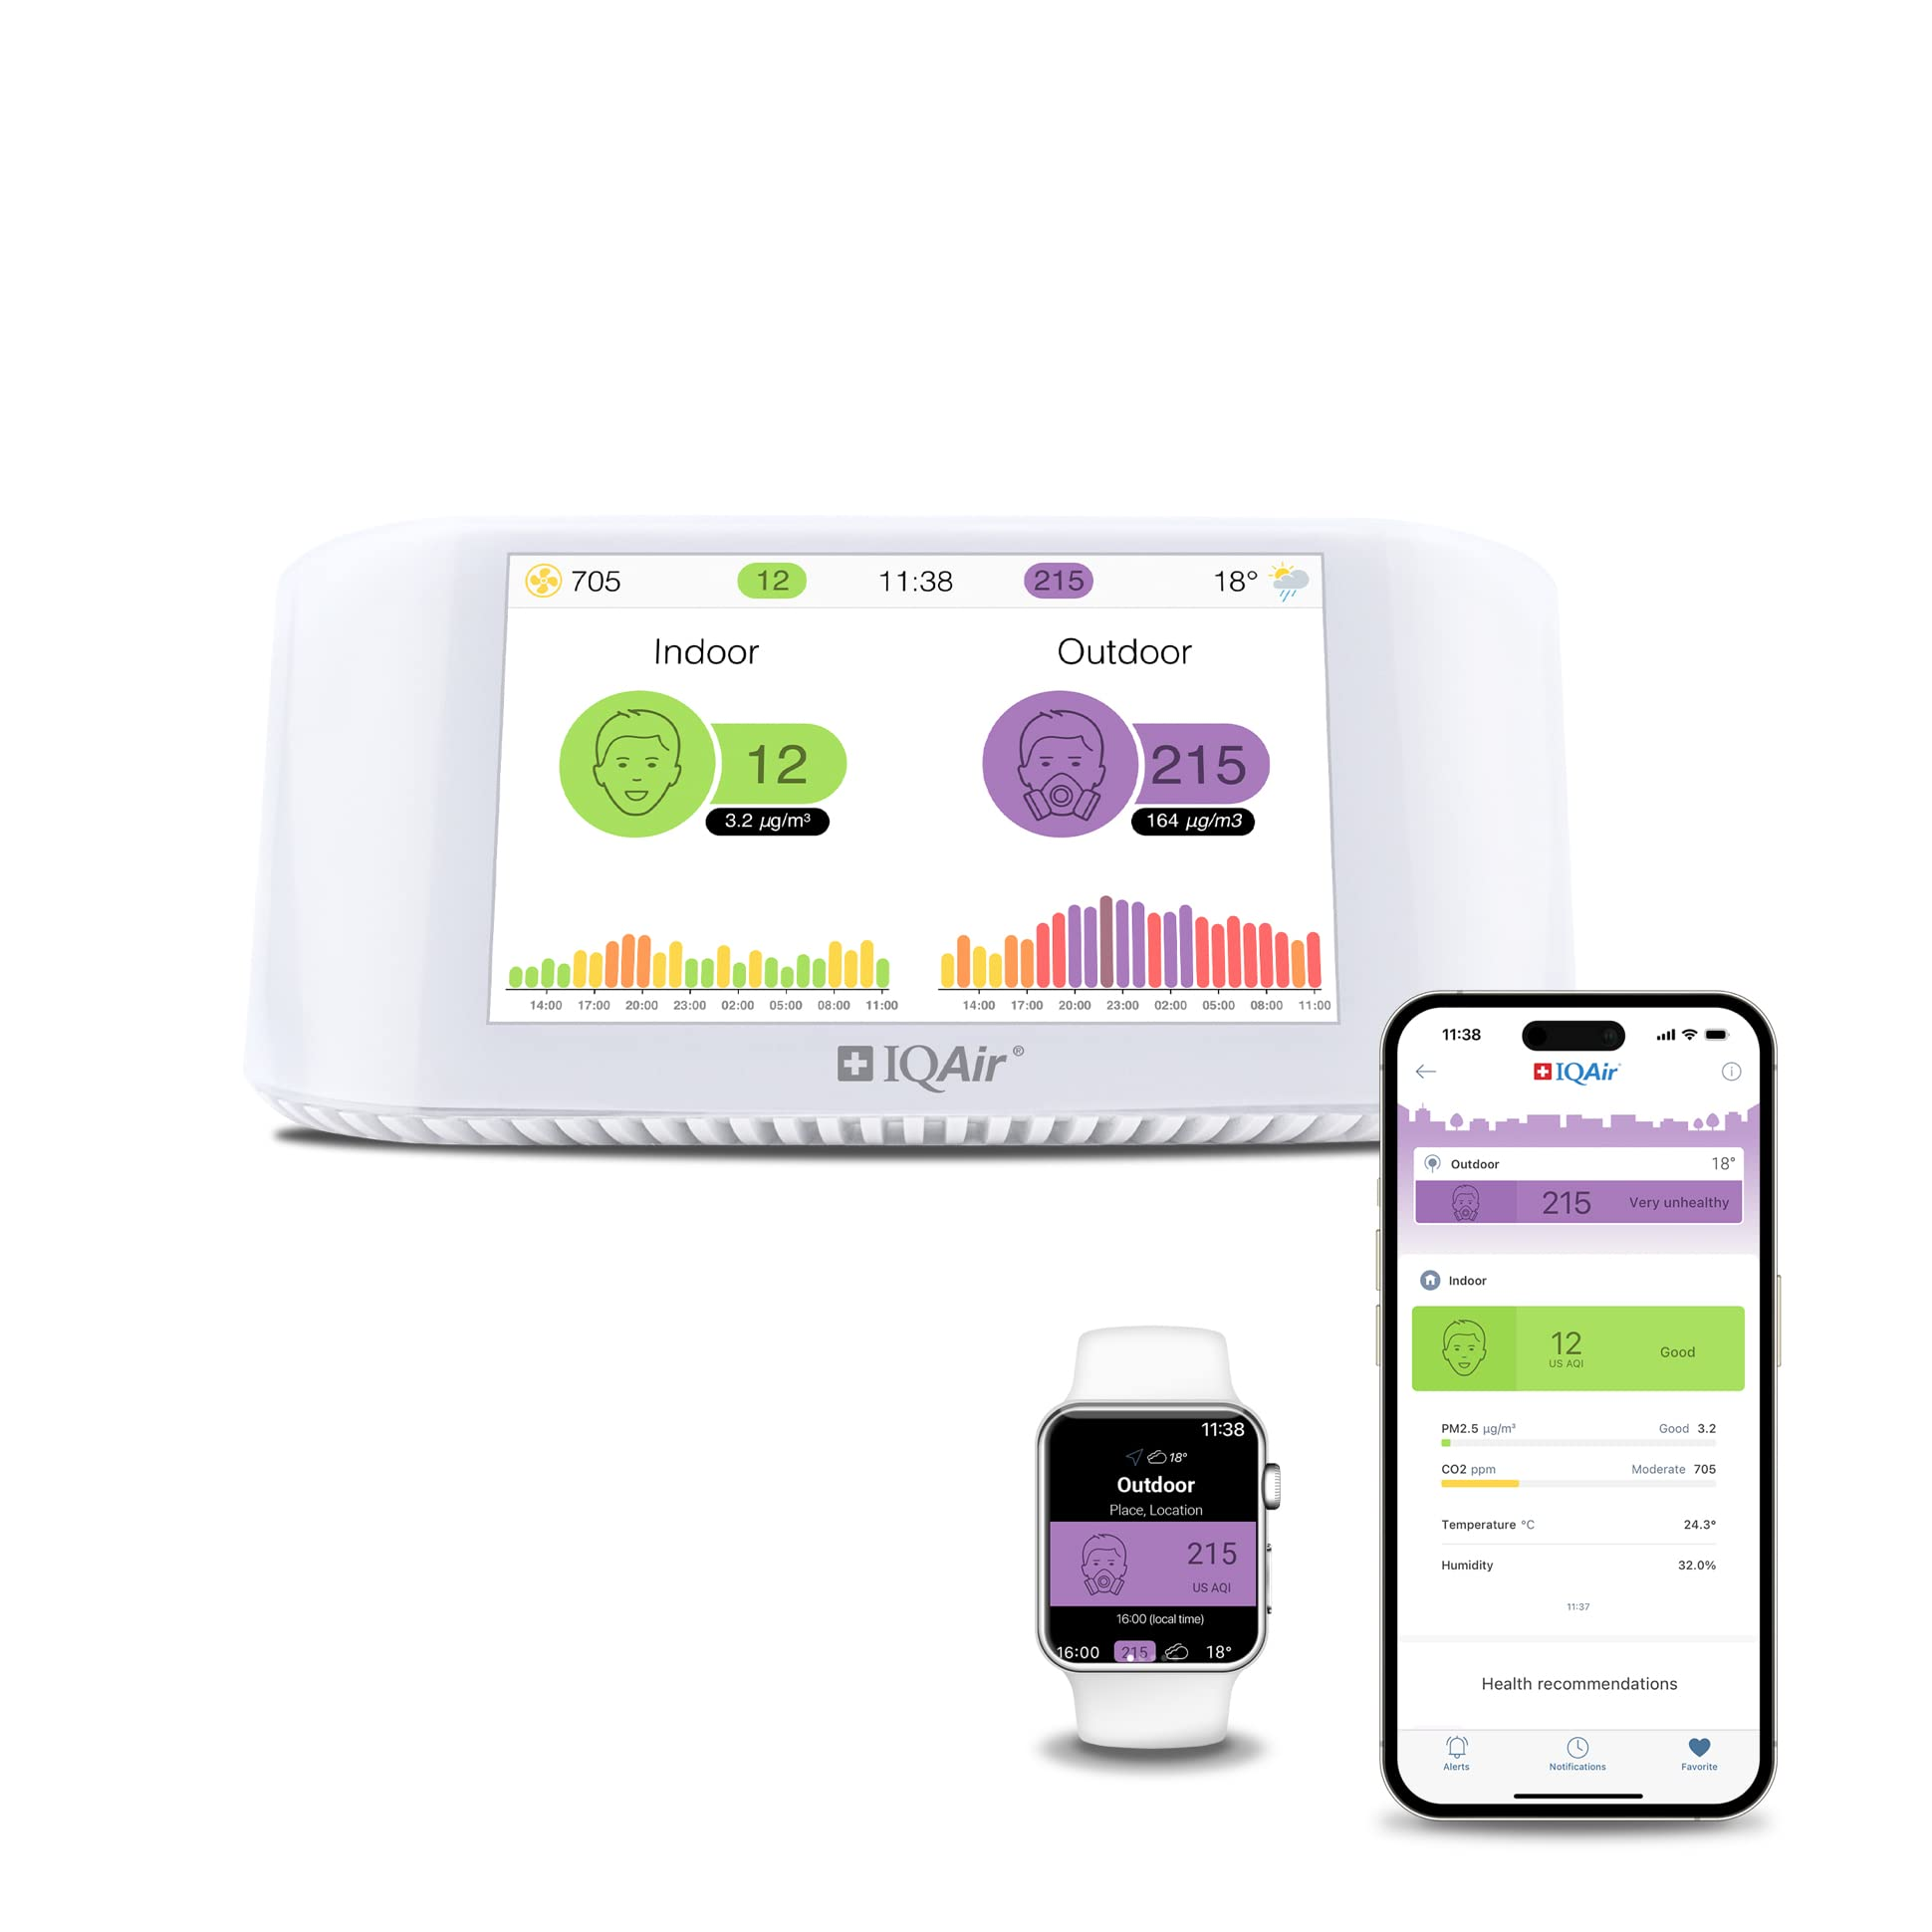
\includegraphics[
        width=0.75\textwidth,
        height=0.28\textheight,
        keepaspectratio
    ]{images/air_quality_pro.jpg}
    \caption{Ví dụ thiết bị đo thương mại di động}
    \label{fig:Thiết bị đo thương mại di động}
\end{figure}

  \begin{itemize}
      \item \textit{Ưu điểm}: Thiết kế thẩm mỹ cao, giao diện hiển thị trực quan đẹp mắt, hỗ trợ đồng bộ ứng dụng di động tốt.
      \item \textit{Hạn chế}: Giá thành cao (khoảng 5 - 8 triệu đồng), không hỗ trợ trích xuất dữ liệu thô dạng bảng dễ dàng cho các bài toán nghiên cứu học máy cục bộ.
    \end{itemize}
    \item \textbf{Hệ thống tự chế DIY/IoT chi phí thấp}:
  \begin{itemize}
      \item \textit{Ưu điểm}: Chi phí linh kiện rất rẻ (< 1 - 2 triệu đồng), cấu trúc mở hoàn toàn, sinh viên có thể tự do lập trình và nâng cấp.
      \item \textit{Hạn chế}: Độ ổn định cơ khí buồng lấy mẫu kém, thường bị mất dữ liệu khi mất kết nối mạng và thiết kế nguồn điện không có mạch bảo vệ chống sụt áp.
    \end{itemize}
\end{itemize}

Bảng \ref{tab:existingsolutions} so sánh tổng quan các nhóm giải pháp trên với nguyên mẫu thiết kế nâng cấp của nhóm.

\begin{table}[H]
\centering
\caption{So sánh nguyên mẫu của nhóm với một số nhóm giải pháp hiện có}
\label{tab:existingsolutions}
\footnotesize
\renewcommand{\arraystretch}{1.35}
\setlength{\tabcolsep}{4pt}

\begin{tabularx}{\textwidth}{|p{3.2cm}|X|X|X|X|}
\hline
\textbf{Tiêu chí so sánh} 
& \textbf{Trạm quan trắc chuyên dụng} 
& \textbf{Thiết bị thương mại} 
& \textbf{Hệ thống DIY cơ bản} 
& \textbf{Nguyên mẫu của nhóm} \\
\hline

Chi phí đầu tư 
& Rất cao, phù hợp triển khai ở quy mô tổ chức hoặc cơ quan chuyên môn 
& Cao, phù hợp người dùng cá nhân có nhu cầu theo dõi chất lượng không khí 
& Thấp, phù hợp học tập và thử nghiệm 
& Thấp, định hướng chi phí sinh viên, linh kiện dễ mua \\
\hline

Mức độ chính xác 
& Cao, có thể sử dụng cảm biến và quy trình đo chuyên dụng 
& Khá cao, phụ thuộc từng dòng sản phẩm 
& Thường chỉ mang tính tham khảo 
& Mang tính tham khảo, tập trung đánh giá xu hướng và kiểm thử hệ thống \\
\hline

Tính mở phần cứng 
& Thấp, hệ thống thường đóng kín 
& Thấp, người dùng khó can thiệp phần cứng 
& Cao, dễ thay đổi linh kiện 
& Cao, có thể thay đổi cảm biến, mạch cảnh báo và khối lấy mẫu khí \\
\hline

Khả năng tùy biến firmware 
& Hạn chế đối với người dùng cuối 
& Hạn chế, phụ thuộc nhà sản xuất 
& Có thể tùy biến nếu người dùng tự lập trình 
& Có, firmware được tổ chức trên ESP32 với FreeRTOS, Mutex và các module riêng \\
\hline

Cơ chế lấy mẫu khí 
& Có thiết kế chuyên dụng, phù hợp đo dài hạn 
& Có vỏ và luồng khí được thiết kế sẵn 
& Thường đặt cảm biến trực tiếp ngoài môi trường 
& Có quạt lấy mẫu khí và khối điều khiển nguồn tải qua relay/MOSFET \\
\hline

Hiển thị tại chỗ 
& Có hoặc tùy hệ thống 
& Có giao diện hiển thị thân thiện 
& Có thể có hoặc không 
& Có màn hình OLED hiển thị dữ liệu và trạng thái hệ thống \\
\hline

Cảnh báo cục bộ 
& Có hoặc tùy cấu hình hệ thống 
& Có, thường qua màn hình hoặc ứng dụng 
& Thường đơn giản hoặc chưa có 
& Có LED và buzzer cảnh báo tại thiết bị \\
\hline

Truyền dữ liệu lên cloud 
& Có thể có trong các hệ thống hiện đại 
& Có, thông qua nền tảng của nhà sản xuất 
& Thường chưa có hoặc triển khai đơn giản 
& Có, ESP32 gửi dữ liệu lên Supabase bằng HTTP POST REST API \\
\hline

Lưu trữ khi mất mạng 
& Có thể có tùy cấu hình 
& Phụ thuộc thiết bị và nền tảng đi kèm 
& Thường không có 
& Có cơ chế offline cache bằng SPIFFS, gửi lại khi mạng phục hồi \\
\hline

Cảnh báo từ xa 
& Có thể có trong hệ thống chuyên dụng 
& Có qua ứng dụng hoặc dịch vụ cloud 
& Thường chưa có 
& Có định hướng Supabase Edge Function kết hợp Telegram Bot; cần cấu hình và kiểm thử triển khai thực tế \\
\hline

Mức độ phù hợp với bài tập lớn 
& Không phù hợp để sinh viên tự triển khai toàn bộ do chi phí và độ phức tạp cao 
& Phù hợp tham khảo, không phù hợp để can thiệp kỹ thuật sâu 
& Phù hợp học tập nhưng thường thiếu tính hệ thống 
& Phù hợp mục tiêu môn học, thể hiện được phần cứng, firmware, cloud và kiểm thử \\
\hline

\end{tabularx}
\end{table}

\subsection{So sánh Supabase HTTP REST với MQTT trong phạm vi project này}
Giao thức truyền thông là yếu tố cốt lõi ảnh hưởng trực tiếp đến hiệu năng và cấu trúc phần mềm của trạm đo IoT. Bảng \ref{tab:httpvsmqtt} phân tích và so sánh việc sử dụng giao thức HTTPS POST trực tiếp lên REST API của Supabase với giao thức MQTT truyền thống trong phạm vi thực tế của project này.

\begin{table}[H]
\centering
\caption{So sánh phương án truyền dữ liệu bằng HTTPS POST và MQTT}
\label{tab:httpvsmqtt}
\footnotesize
\renewcommand{\arraystretch}{1.35}
\setlength{\tabcolsep}{5pt}

\begin{tabularx}{\textwidth}{|p{3.3cm}|X|X|}
\hline
\textbf{Tiêu chí so sánh} 
& \textbf{HTTPS POST trực tiếp tới Supabase} 
& \textbf{MQTT thông qua Broker trung gian} \\
\hline

Kiến trúc hệ thống 
& ESP32 gửi dữ liệu trực tiếp tới Supabase thông qua REST API. Kiến trúc đơn giản, không cần triển khai thêm server trung gian để nhận và ghi dữ liệu. 
& ESP32 publish dữ liệu lên MQTT Broker. Để lưu vào cơ sở dữ liệu, hệ thống thường cần thêm một subscriber hoặc backend service trung gian. \\
\hline

Độ phức tạp triển khai 
& Thấp hơn trong phạm vi bài tập lớn. Nhóm chỉ cần cấu hình endpoint, API key và định dạng JSON phù hợp với bảng dữ liệu. 
& Cao hơn do cần cấu hình broker, topic, subscriber, cơ chế ghi cơ sở dữ liệu và xử lý lỗi giữa nhiều thành phần. \\
\hline

Overhead truyền dữ liệu 
& Lớn hơn do có HTTP header và quá trình thiết lập kết nối bảo mật. Phù hợp hơn với chu kỳ gửi dữ liệu không quá dày. 
& Nhỏ hơn, phù hợp với các hệ thống cần gửi dữ liệu thường xuyên hoặc nhiều node cảm biến hoạt động đồng thời. \\
\hline

Khả năng lưu trữ dữ liệu 
& Dữ liệu có thể được ghi trực tiếp vào bảng trong Supabase/PostgreSQL sau mỗi request hợp lệ. Điều này giúp đơn giản hóa luồng dữ liệu từ thiết bị lên cloud. 
& MQTT chỉ đảm nhiệm truyền thông publish/subscribe. Việc lưu trữ vào database cần được thực hiện bởi một thành phần khác như backend service hoặc subscriber. \\
\hline

Bảo mật 
& Hỗ trợ HTTPS/TLS và xác thực bằng API key hoặc Bearer Token. Tuy nhiên, cần bảo vệ khóa truy cập và không đưa secret nhạy cảm vào firmware public. 
& Có thể hỗ trợ TLS và cơ chế xác thực broker. Tuy nhiên, việc cấu hình bảo mật đầy đủ trên thiết bị nhúng và broker cần được triển khai cẩn thận. \\
\hline

Khả năng mở rộng 
& Phù hợp với nguyên mẫu ít node, tần suất gửi dữ liệu vừa phải và cần lưu dữ liệu trực tiếp lên cloud. 
& Phù hợp hơn khi hệ thống có nhiều node, cần truyền dữ liệu thời gian thực, publish/subscribe hoặc điều khiển hai chiều. \\
\hline

Xử lý khi mất mạng 
& Trong đề tài, ESP32 kết hợp HTTPS POST với cơ chế offline cache bằng SPIFFS. Khi mất Wi-Fi hoặc gửi thất bại, dữ liệu được lưu tạm và gửi lại sau. 
& MQTT có thể hỗ trợ QoS và session tùy cấu hình broker/client, nhưng vẫn cần thiết kế thêm cơ chế lưu cục bộ nếu muốn chống mất dữ liệu hoàn toàn khi thiết bị mất mạng lâu. \\
\hline

Mức độ phù hợp với đề tài 
& Phù hợp với nguyên mẫu của nhóm: hệ thống gửi dữ liệu theo chu kỳ, ưu tiên kiến trúc đơn giản, dễ tích hợp với Supabase và dễ trình bày trong báo cáo. 
& Phù hợp với hệ thống IoT nhiều node hoặc yêu cầu truyền nhận liên tục. Trong phạm vi đề tài hiện tại, MQTT làm tăng số thành phần cần triển khai. \\
\hline

Kết luận lựa chọn 
& Được nhóm lựa chọn vì đơn giản, trực tiếp, phù hợp với Supabase và giảm khối lượng triển khai backend. 
& Được xem là phương án mở rộng nếu hệ thống phát triển thành mạng nhiều node cảm biến hoặc cần giao tiếp thời gian thực hơn. \\
\hline

\end{tabularx}
\end{table}

\section{Tổng quan chức năng hệ thống}
\subsection{Các tác nhân hệ thống (Actors)}
Hệ thống quan trắc chất lượng không khí tương tác với 4 tác nhân chính:
\begin{enumerate}
    \item \textbf{Người phát triển / Sinh viên (Developer)}: Cấu hình phần cứng, nạp firmware, theo dõi log debug qua Serial Monitor, trích xuất dữ liệu lịch sử để chạy thuật toán hiệu chuẩn.
    \item \textbf{Người quan sát / Người dùng (Observer)}: Theo dõi các chỉ số đo trực quan tại chỗ qua màn hình OLED hoặc nhận tin nhắn báo cáo/cảnh báo trên điện thoại qua Telegram.
    \item \textbf{Cơ sở dữ liệu Supabase (Cloud Database)}: Lưu trữ dữ liệu đo đạc, thực thi các database webhooks để kích hoạt Edge Functions.
    \item \textbf{Telegram Bot API (Alerting Service)}: Tiếp nhận yêu cầu gửi tin nhắn từ Edge Function và chuyển tiếp tin nhắn cảnh báo tới chat ID của người dùng.
\end{enumerate}

\subsection{Sơ đồ Use Case tổng quát}
Mối quan hệ tương tác giữa các tác nhân và chức năng hệ thống được mô tả khái quát qua biểu đồ use case dưới đây.

\begin{figure}[H]
    \centering
    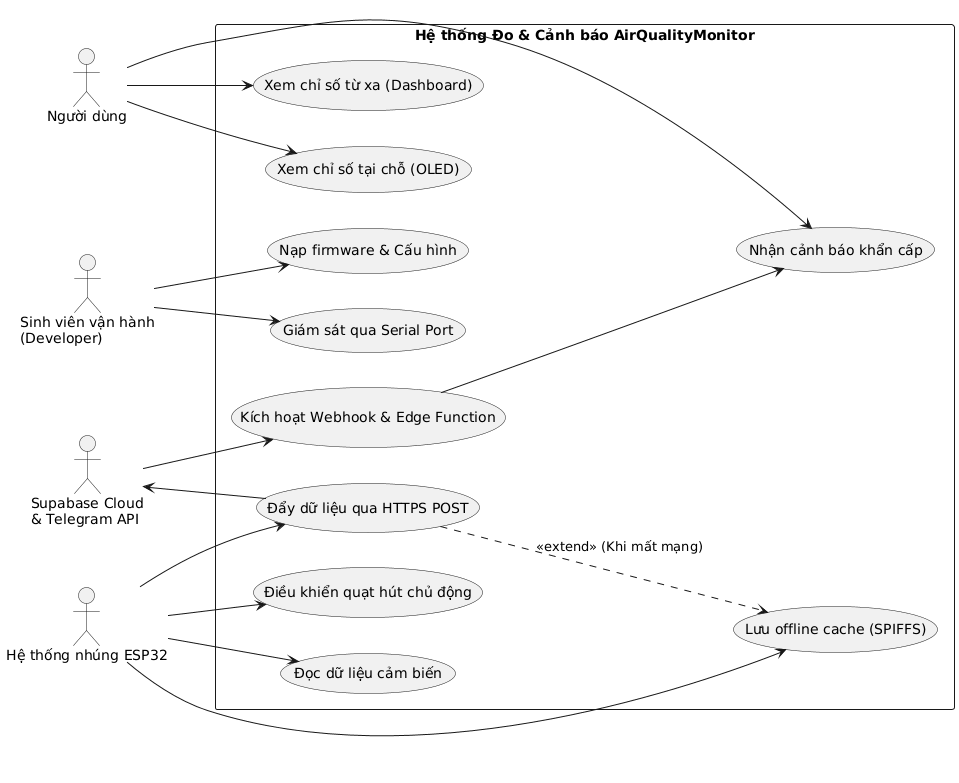
\includegraphics[
        width=0.95\textwidth,
        height=0.55\textheight,
        keepaspectratio
    ]{images/use_case_tong_quan.png}
    \caption{Biểu đồ Use Case tổng quát của hệ thống}
    \label{fig:usecase}
\end{figure}

\subsection{Quy trình vận hành tổng quát}
Quy trình hoạt động của trạm đo chất lượng không khí bắt đầu ngay khi thiết bị được cấp nguồn:
\begin{enumerate}
    \item \textbf{Khởi tạo hệ thống}: ESP32 bật nguồn, khởi tạo cổng Serial, cấu hình chân GPIO, gắn ngắt ngoài cho nút bấm, khởi tạo bus I2C điều khiển OLED, khởi tạo cảm biến và nạp dữ liệu cấu hình từ SPIFFS.
    \item \textbf{Chu kỳ làm nóng cảm biến (Warm-up State)}: Relay kích hoạt cấp nguồn 5V cho buồng đo, quạt hút bắt đầu chạy và dây gia nhiệt của MQ135 hoạt động. Màn hình OLED hiển thị trạng thái đếm ngược 60 giây để cảm biến ổn định nhiệt độ.
    \item \textbf{Đọc cảm biến (Read State)}: Sau 60 giây, ESP32 bật LED hồng ngoại của GP2Y1010, đọc giá trị điện áp ADC từ cảm biến bụi và khí MQ135, đồng thời đọc nhiệt độ/độ ẩm từ DHT22.
    \item \textbf{Cập nhật và Cảnh báo cục bộ}: Dữ liệu được lọc nhiễu, cập nhật lên màn hình OLED. Nếu các chỉ số vượt ngưỡng cấu hình an toàn, còi buzzer và LED đỏ sẽ phát tín hiệu cảnh báo.
    \item \textbf{Truyền dữ liệu đám mây (Publish State)}: TaskNetwork kiểm tra kết nối Wi-Fi. Nếu có mạng, dữ liệu được đóng gói JSON và POST lên Supabase, đồng thời quét và gửi bù dữ liệu lưu trong SPIFFS cache (nếu có). Nếu mất mạng, dữ liệu tự động ghi vào file \texttt{/cache.txt} trong SPIFFS.
    \item \textbf{Trạng thái chờ (Idle State)}: Tắt Relay cấp nguồn buồng đo và quạt hút (RELAY\_OFF) để tiết kiệm năng lượng và tăng tuổi thọ cảm biến, sau đó hệ thống ngủ trong 5 phút trước khi lặp lại chu kỳ mới.
\end{enumerate}

\section{Yêu cầu chức năng (Functional Requirements)}
Các yêu cầu chức năng bắt buộc đối với trạm quan trắc chất lượng không khí được mô tả chi tiết trong Bảng \ref{tab:functionalreqs}.

\begin{table}[H]
\centering
\caption{Bảng yêu cầu chức năng hệ thống (FR)}
\label{tab:functionalreqs}
\small
\renewcommand{\arraystretch}{1.35}
\setlength{\tabcolsep}{6pt}

\begin{tabularx}{\textwidth}{|c|p{3.2cm}|X|}
\hline
\textbf{ID} & \textbf{Tên yêu cầu} & \textbf{Mô tả chi tiết tính năng} \\
\hline

\textbf{FR1} & Đo lường chỉ số & 
Hệ thống phải tự động đo các thông số nhiệt độ, độ ẩm, nồng độ bụi tương đối, nồng độ khí gas tổng quát và áp suất khí quyển. \\
\hline

\textbf{FR2} & Làm nóng cảm biến & 
Hệ thống phải điều khiển relay bật nguồn quạt hút và bộ nung cảm biến khí ổn định trước khi đọc dữ liệu 60 giây. \\
\hline

\textbf{FR3} & Hiển thị trực quan & 
Hệ thống phải hiển thị trạng thái hoạt động, quá trình đếm ngược warm-up, các thông số đo được và địa chỉ IP Wi-Fi lên OLED SSD1306. \\
\hline

\textbf{FR4} & Cảnh báo tại chỗ & 
Phát tín hiệu còi buzzer kêu ngắt quãng và nháy LED đỏ liên tục khi bất kỳ chỉ số nào vượt ngưỡng cảnh báo thiết lập. \\
\hline

\textbf{FR5} & Gửi dữ liệu đám mây & 
Đóng gói dữ liệu dạng JSON và thực hiện HTTP POST an toàn (có Bearer Token) lên cơ sở dữ liệu Supabase qua Wi-Fi. \\
\hline

\textbf{FR6} & Offline Caching & 
Tự động phát hiện mất mạng, chuyển đổi trạng thái lưu trữ cục bộ vào flash qua SPIFFS, và đẩy bù dữ liệu khi mạng được khôi phục. \\
\hline

\textbf{FR7} & Cảnh báo từ xa & 
Gửi tin nhắn cảnh báo tiếng Việt không dấu đến Telegram của người dùng ngay lập tức khi phát hiện khí gas rò rỉ hoặc bụi mịn vượt ngưỡng. \\
\hline

\end{tabularx}
\end{table}

\section{Yêu cầu phi chức năng (Non-Functional Requirements)}
Bên cạnh các tính năng cốt lõi, trạm đo cần đáp ứng các tiêu chuẩn kỹ thuật phi chức năng về hiệu năng, độ ổn định và chi phí được tổng hợp trong Bảng \ref{tab:nonfunctionalreqs}.

\begin{table}[H]
\centering
\caption{Bảng yêu cầu phi chức năng hệ thống (NFR)}
\label{tab:nonfunctionalreqs}
\small
\renewcommand{\arraystretch}{1.35}
\setlength{\tabcolsep}{5pt}

\begin{tabularx}{\textwidth}{|c|p{3.0cm}|X|p{2.6cm}|}
\hline
\textbf{ID} & \textbf{Nhóm yêu cầu} & \textbf{Mô tả chi tiết yêu cầu kỹ thuật} & \textbf{Chỉ tiêu đạt} \\
\hline

\textbf{NFR1} & Thời gian đáp ứng & 
Thời gian cập nhật OLED sau khi đọc cảm biến hoàn tất. 
& $< 1$ giây \\
\hline

\textbf{NFR2} & Độ trễ truyền cloud & 
Độ trễ gửi HTTP POST lên Supabase khi mạng ổn định. 
& $< 2$ giây \\
\hline

\textbf{NFR3} & Thời gian giữ cache & 
Hệ thống phải lưu trữ dữ liệu offline liên tục trong nhiều ngày khi mất Wi-Fi. 
& Tối thiểu 7 ngày \\
\hline

\textbf{NFR4} & Độ ổn định phần mềm & 
Hệ thống phải chạy liên tục không bị treo đơ nhờ cơ chế Watchdog Timer. 
& 24/7 không lỗi \\
\hline

\textbf{NFR5} & Tiết kiệm năng lượng & 
Tắt nguồn buồng đo và quạt hút trong trạng thái IDLE. 
& Giảm dòng tiêu thụ \\
\hline

\textbf{NFR6} & Tính phi chặn (Non-blocking) & 
Mạng lỗi hoặc mất kết nối cloud không được làm treo task đọc cảm biến hay task OLED. 
& Sử dụng FreeRTOS \\
\hline

\textbf{NFR7} & An toàn dữ liệu & 
Ngăn chặn tranh chấp ghi đọc SensorRecord bằng cơ chế khóa bảo vệ. 
& Dùng \texttt{dataMutex} \\
\hline

\textbf{NFR8} & Tránh xung đột I2C & 
Tránh xung đột khi cả task đọc cảm biến và task OLED truy cập bus I2C cùng lúc. 
& Dùng \texttt{i2cMutex} \\
\hline

\textbf{NFR9} & Tính bảo mật token & 
Giấu kín hoàn toàn Telegram Bot Token khỏi firmware của thiết bị. 
& Dùng Edge Functions \\
\hline

\textbf{NFR10} & Chi phí chế tạo & 
Tổng chi phí linh kiện phần cứng cho một nút đo nguyên mẫu. 
& $< 2.000.000$ VNĐ \\
\hline

\textbf{NFR11} & Khả năng mở rộng & 
Dễ dàng tích hợp thêm cảm biến mới hoặc thay đổi chu kỳ mà không cần viết lại toàn bộ code. 
& Thiết kế module hóa \\
\hline

\textbf{NFR12} & Khả năng cập nhật & 
Hỗ trợ nạp chương trình từ xa thông qua mạng Wi-Fi nội bộ. 
& Cấu hình OTA thành công \\
\hline

\end{tabularx}
\end{table}